%! TEX root = ../main.tex
\documentclass[main]{subfiles}

\begin{document}
\chapter{先行研究の概要}
    本研究内容の元となる,先行研究の概要をまとめる\cite{senkoukenkyu}.

    \section{長野駅中心モデルのシナリオ}
    長野市において路線バスの多くが発着する長野駅を中心とした地域をシミュレーションする.
    長野市のバス利用率を4.5\%,10\%,15\%に設定しそれぞれで最適化を行い,得られるパレート最適解集合の性質を検証する.

    \section{Hypervolume(HV)}
    多目的最適化のパレート最適解集合を評価するための指標としてHypervolumeを用いる\cite{hv}.
    HVはパレート最適解の収束性と多様性を測る.
    HVは,あらかじめ設定する参照点\boldmath$r$と,得られたパレート最適解集合が目的空間で形成する
    M次元体積を求めたものである.ここで,Mは目的数を表す.
    HVは図\ref{hv_siki}で求められる.
    \begin{align}
        v(\bf{p}^{(j)}, \bf r) = \prod_{i=1}^d (r_i - p_i^{(j)}) \\
        HV = \bigcup_{j=1}^n v(\bf{p}^{(j)}, \bf r)
        \label{hv_siki}
    \end{align}
    M目的最適化問題の時,参照点\boldmath$r$はパレート最適解集合中のどの解が持つ各目的関数値よりも悪い点に設定する.
    HVはこの参照点\boldmath$r$とパレート最適解集合を囲む領域である.
    HVの値が大きいほど,収束性が高く,多様性のあるパレート最適解集合であると言える.
    式\ref{hv_image}に2目的最小化問題の時のHVの概要を示す.

    \begin{figure}
        \centering
        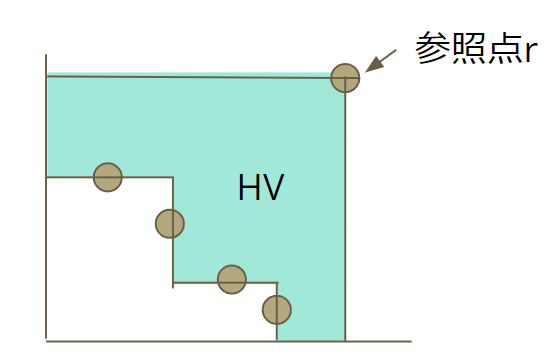
\includegraphics[width=\linewidth]{figures/hv_image.png}
        \caption{HVの概要}
        \label{hv_image}
    \end{figure}

    \section{結果}\label{senkoukekka}
    遺伝的アルゴリズムの世代ごとにHVをプロットしたグラフを図\ref{hv_plot}に示す.
    先行研究ではバス利用率4.5\%,10\%,15\%の場合のHV推移を求めていたが,ここでは本研究に用いる4.5\%の結果のみ示す.

    \begin{figure}
        \centering
        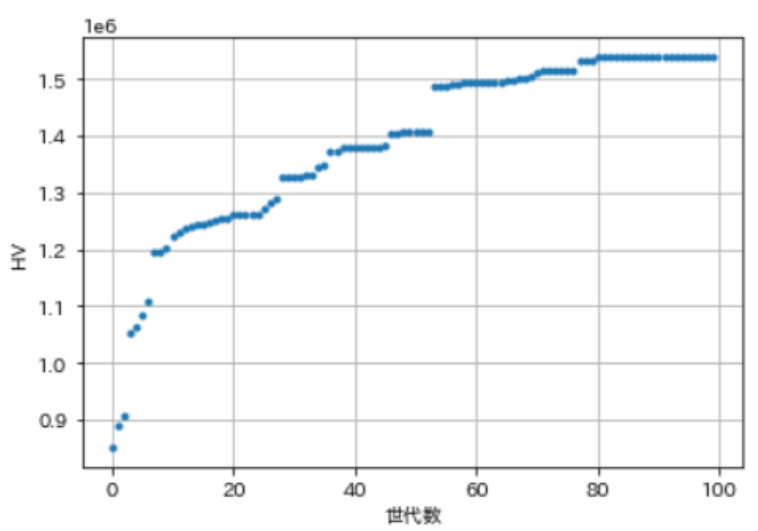
\includegraphics[width=\linewidth]{figures/hv_plot.png}
        \caption{バス利用率4.5\%の場合のHV推移}
        \label{hv_plot}
    \end{figure}

    バス利用率を複数設定し,そのHV推移の結果から
    \begin{itemize}
        \item それぞれの利用率で最適化が行われている
        \item 総移動時間-乗車率にはトレードオフの関係が存在する
        \item バス利用率と総移動時間,バス利用率と乗車率の間には比例の関係が存在する
    \end{itemize}
    ことが分かった.

    \section{先行研究の課題点}
    先行研究の課題点として計算時間が大変長いという点が上げられる.
    先行研究では,1つの運行計画をSUMOによりシミュレートすると約40分かかる.
    実験では1世代に20個体生成し,100世代分繰り返しているため,計算時間は$20\times 100\times 40 = 80000分 \fallingdotseq 2ヶ月$となる.
    実際にバス運行スケジュールを決定するにあたり,2ヶ月をかけるのはバス運行会社としては非現実的である.

\end{document}

